% cvicenie 1

\documentclass{beamer}

\mode<presentation>
{
  %\usetheme{Warsaw}
  %\usetheme{Singapore}
  %\usetheme{Szeged}
  \usetheme{Boadilla}

  \setbeamercovered{transparent}
  % or whatever (possibly just delete it)
}
\input newcomm
%\usepackage{slovak}
\usepackage{times}
\usepackage{psfrag}
\usepackage{graphics}
\usepackage{amsfonts}
\usepackage{amssymb}
\usepackage{amsmath}
\usepackage{theorem}
\usepackage{subfigure}
\usepackage{epsfig}
%\usepackage{natbib}
\usepackage{mathrsfs} %mathscr
\usepackage[cp1250]{inputenc}
\usepackage[T1]{fontenc}
\usepackage{listings}
\usepackage{multirow}
\usepackage{epstopdf}

\usepackage{amsmath}
\usepackage{amssymb}
\renewcommand{\vec}[1]{\boldsymbol{#1}} %I want bold vectors instead of arrows
\newcommand{\tab}[1]{\hspace{.1\textwidth}\rlap{#1}}

\title[TAR III.] % (optional, use only with long paper titles)
{Te�ria automatick�ho riadenia III.}
\subtitle{Cvi�enie V, K�lm�nov filter, pokra�ovanie}

\author[] % (optional, use only with lots of authors)
{G. Tak�cs, G. Batista}


\institute[UAMAI] % (optional, but mostly needed)
{
  �stav automatiz�cie, merania a aplikovanej informatiky\\
  Strojn�cka fakulta, Slovensk� technick� univerzita}
%  \and
%  \inst{2}%
%  Department of Theoretical Philosophy\\
%  University of Elsewhere}
% - Use the \inst command only if there are several affiliations.
% - Keep it simple, no one is interested in your street address.

\date[24.10.2016] % (optional, should be abbreviation of conference name)
{}
% - Either use conference name or its abbreviation.
% - Not really informative to the audience, more for people (including
%   yourself) who are reading the slides online

\subject{Automatiz�cia a riadenie}
% This is only inserted into the PDF information catalog. Can be left
% out.

%\begin{center}
%\includegraphics[height=2cm]{logo_stu_sjf_clr.eps} \\
%\end{center}

% If you have a file called "university-logo-filename.xxx", where xxx
% is a graphic format that can be processed by latex or pdflatex,
% resp., then you can add a logo as follows:

%\pgfdeclareimage[height=1.5cm]{logo}{logo}
%\logo{\pgfuseimage{logo}}



% Delete this, if you do not want the table of contents to pop up at
% the beginning of each subsection:
%\AtBeginSubsection[]
%{
%  \begin{frame}<beamer>{Obsah}
%    \tableofcontents[currentsection,currentsubsection]
%  \end{frame}
%}

\begin{document}
\setbeamertemplate{caption}{\raggedright\insertcaption\par}

\begin{frame}
  \titlepage
\end{frame}

\begin{frame}{Probl�m}
\begin{columns}[T]

\begin{column}{0.48\textwidth}
\begin{figure}
\centering
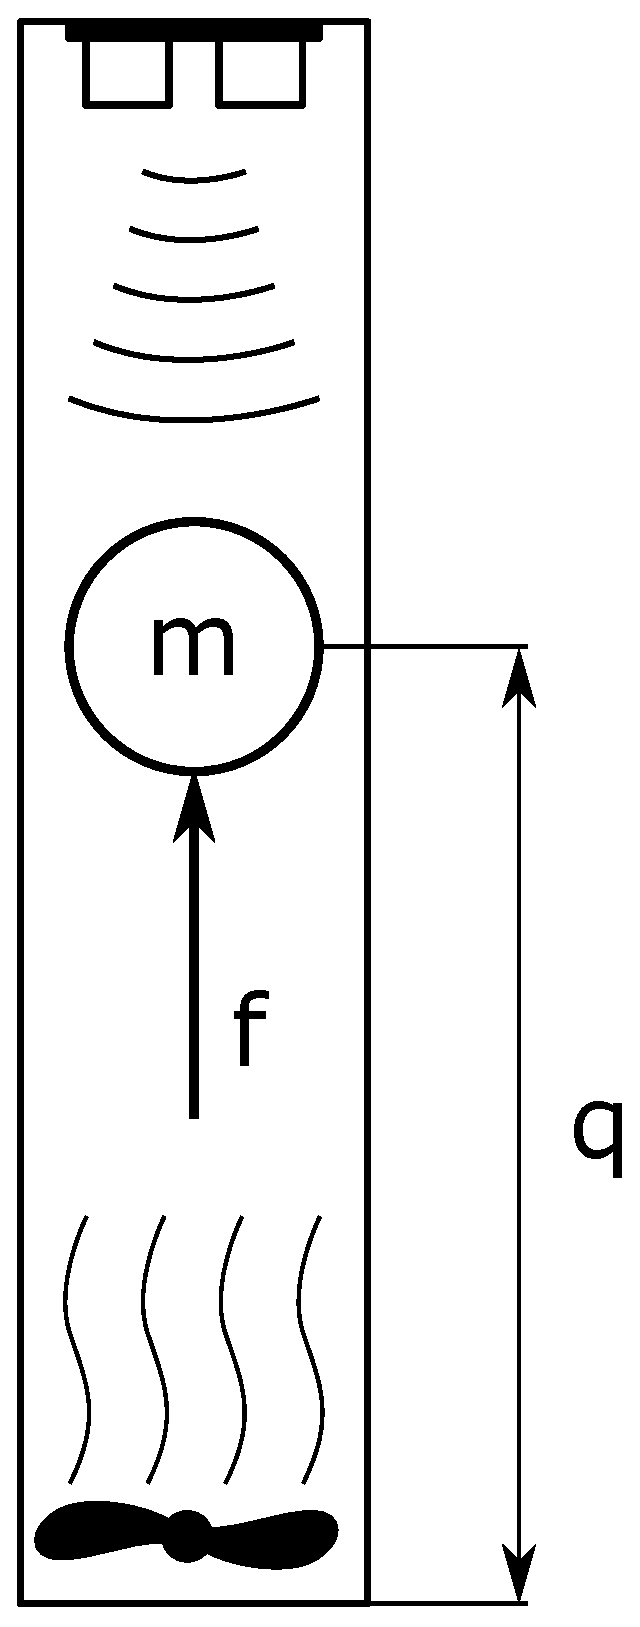
\includegraphics[width = 2cm]{ventilator.eps}
\end{figure}
\end{column}

\begin{column}{0.48\textwidth}
Model syst�mu:
\begin{eqnarray*}
\ddot{q} &=& \frac{1}{m}f \hspace{0.3cm} \vline \hspace{0.3cm} \frac{d}{dt}\\
\dddot{q} &=& \frac{1}{m}\dot{f}\\
\end{eqnarray*}

\begin{eqnarray*}
\begin{bmatrix}
\dot{q}\\
\ddot{q}\\
\dddot{q}\\
\end{bmatrix}
=
\begin{bmatrix}
0 & 1 & 0\\
0 & 0 & 1\\
0 & 0 & 0\\
\end{bmatrix}
\begin{bmatrix}
q\\
\dot{q}\\
\ddot{q}\\
\end{bmatrix}
+
\begin{bmatrix}
0\\
0\\
\frac{1}{m}\\
\end{bmatrix}
\dot{f}\\
\end{eqnarray*}

\end{column}
\end{columns}

\end{frame}

\begin{frame}{Nastavenia}

Zostav�me K�lm�nov filter pre 3 r�zne konfigur�cie merania:

\begin{itemize}
\item
\begin{equation*}
C = 
\begin{bmatrix}
1 & 0 & 0\\
0 & 0 & 1
\end{bmatrix}
\end{equation*}

\item
\begin{equation*}
C = 
\begin{bmatrix}
1 & 0 & 0
\end{bmatrix}
\end{equation*}

\item
\begin{equation*}
C = 
\begin{bmatrix}
0 & 0 & 1
\end{bmatrix}
\end{equation*}

\end{itemize}

\end{frame}

\begin{frame}{�loha}
�lohou dne�n�ho cvi�enia je vy�etri� spr�vanie sa K�lm�novho filtra pre:

\begin{itemize}
\item Odhad stavu so sp�tnou v�zbou vstupu
\item Odhad stavu bez sp�tnej v�zby vstupu
\item Odhad stavu pri nekoreknom ur�en� po�iato�n�ho stavu syst�mu
\end{itemize}

\end{frame}

\end{document}